\chapter{Smart Elasticity}
\label{chp:smart-elasticity}


% %
% HEADER
% %
The smart elasticity is the ability of a system to dynamically auto-scale resources according to scaling policies determined with machine learning techniques.
%
The smart elasticity service hence provides a resource manager, e.g. a container orchestrator, with the ability to learn the best replication degree for its resources, e.g. deployed containers, with respect to the current cluster state.
%
In this work we propose to implement smart elasticity for Kubernetes leveraging reinforcement learning, that is the most famous technique of unsupervised machine learning.
%
In particular, we focus on $\mathcal{Q}$-Learning, which is the most widely studied reinforcement learning algorithm.
%
In this Chapter we show the adopted reinforcement learning model, the pseudocode of the learning algorithm that realizes it and the implementation of the overall service.

%
%First, we exlain how the general Q-Learning algorithm can be adapted to achieve smart elasticity. In particulr, we show the pseudocode that implements the algorithm.
%
%Then, we show how the smart elasticity service has been implemented in the Kubernetes environment. 
%In particular, we show the reference architecture, component interactions and the REST interfaces.


% %
% ELASTICITY LEVERAGING Q-LEARNING
% %
\section{Elasticity leveraging $\mathcal{Q}$-Learning}
\label{sec:smart-elasticity-elasticity-leveraging-q-learning}

A reinforcement learning algorithm can be used to learn the best scaling policy to adopt in response to cluster state changes without any past knowledge.
%
In this work, we propose an approach that makes use of the $\mathcal{Q}$-Learning algorithm, described in Chapter \ref{chp:reinforcement-learning}.
%
A general $\mathcal{Q}$-Learning algorithm relies on a reinforcement learning model that requires the definition of the following spaces, functions and parameters:

\begin{itemize}
	
	\item State Space $\mathcal{S}$ where each state $s\in\mathcal{S}$ is a cluster state.
	
	\item Action Space $\mathcal{A}$ where each action $a\in\mathcal{A}$ is a scaling action.
	
	\item Quality Function $\mathcal{Q}:\mathcal{S}\times\mathcal{A}\rightarrow\Re$ where the value $q_{s_{t},a_{t}}=\mathcal{Q}(s_{t},a_{t})$ is the quality of performing the action $a_{t}$ in the state $s_{t}$ at time $t$.
	%
	Notice that, since Q-Learning is an iterative algorithm that updates $\mathcal{Q}$, this function requires an initialization setting $\mathcal{Q}_{0}$.
	
	\item Rewarding Function $\mathcal{R}:\mathcal{S}\rightarrow\Re$ where the value $r_{t}=\mathcal{R}(s_{t})$ is the rewarding achieved for the state $s_{t}$.
	
	\item Learning Rate $\alpha\in (0,1]$ that trades off the importance of sooner versus later quality values 
	
	\item Discount Factor $\gamma\in [0,1]$ that trades off the importance of sooner versus later rewards.
\end{itemize}

These items encapsulate the peculiarities of the domain where the algorithm is applied and are used by the Agent to determine the optimality of an action in a state, according to the following update:

\begin{equation}
	\label{eqn:smart-elasticity-reinforcement-learning-update}
	\mathcal{Q}(s_{t},a_{t}) \leftarrow (1-\alpha) \cdot \mathcal{Q}(s_{t},a_{t}) + \alpha \cdot (r_{t} + \gamma \cdot \max_{a}(\mathcal{Q}(s_{t+1},a_{t}))
\end{equation}

In the following, we show and motivate our choice for the aforementioned parameters in the context of smart elasticity.


\subsection{State Space}
\label{sec:smart-elasticity-elasticity-leveraging-q-learning-state-space}

INSERT HERE DESCRIPTION OF THE STATE SPACE (ITERATE WITH PROF).


\subsection{Action Space}
\label{sec:smart-elasticity-elasticity-leveraging-q-learning-action-space}

INSERT HERE THE DESCRIPTION AND MOTIVATIONS OF THE CHOOSEN ACTION SPACE (ITERATE WITH PROF).


\subsection{Quality Function}
\label{sec:smart-elasticity-elasticity-leveraging-q-learning-quality-function}

INSERT HERE THE DESCRIPTION AND MOTIVATIONS OF THE CHOOSEN QUALITY FUNCTION (ITERATE WITH PROF).


\subsection{Rewarding Function}
\label{sec:smart-elasticity-elasticity-leveraging-q-learning-rewarding-function}

INSERT HERE THE DESCRIPTION AND MOTIVATIONS OF THE CHOOSEN REWARDING FUNCTION (ITERATE WITH PROF).


\subsection{Learning Rate}
\label{sec:smart-elasticity-elasticity-leveraging-q-learning-learning-rate}

INSERT HERE THE DESCRIPTION AND MOTIVATIONS OF THE CHOOSEN LEARNING RATE (ITERATE WITH PROF).


\subsection{Discount Factor}
\label{sec:smart-elasticity-elasticity-leveraging-q-learning-discount-factor}

INSERT HERE THE DESCRIPTION AND MOTIVATIONS OF THE CHOOSEN DISCOUNT FACTOR (ITERATE WITH PROF).


% %
% ALGORITHM
% %
\section{Algorithm}
\label{sec:smart-elasticity-algorithm}

INSERT HERE A DETAILED DESCRIPTION OF THE PSEUDOCODE IN ALGORITHM \ref{alg:smart-elasticity-algorithm}.

\begin{algorithm}[t]
	\label{alg:smart-elasticity-algorithm}
	\SetKwProg{Fn}{Function}{}{}  
	
	\Fn{foo (bar)} {
		$print "Hello World"$ \\
	}
	\caption{Pseudocode of the \texttt{SmartElasticity} algorithm.}
\end{algorithm}


% %
% IMPLEMENTATION
% %
\section{Implementation}
\label{sec:smart-elasticity-implementation}

The smart elasticity service is realized by the following four main components, interacting via REST interfaces.
%
In Figure \ref{fig:smart-elasticity-architecture} we show the high-level reference architecture for the smart elasticity service, represented as a UML component diagram.

\begin{itemize}
	
	\item \texttt{ClusterMonitor} collects cluster performance metrics focused on CPU, Memory and Network utilization in a per-node and/or per-container basis. 
	%
	These metrics can be queried via a REST interface.
	%
	In a usual Kubernetes cluster, this component is realized by the Heapster master.
	
	\item \texttt{Orchestrator} responsible for containers orchestration. 
	%
	In particular, it deployes containers and dynamically scales them in/out accordingly with the scaling actions provided by the \texttt{ScalerAI}.
	%
	It pulls \texttt{ScalerAI} at fixed time interval to retrieve the scaling action to perform with respect to the current cluster state. 
	%
	Since the smart elasticity service can be provided to distinct cluster contexts, a token is required to identify the context during REST inetractions.
	%
	In a usual Kubernetes cluster, this component is realized by the Kubernetes leading master.
	
	\item \texttt{ScalerAI} responsible for the smart elasticity service.
	%
	In particular it determines the best scaling action with respect to the current cluster state accordingly to the adopted reinforcement learning technique. 
	%
	It exposes a REST interface through which the \texttt{Orchestrator} can ask for scaling actions.
	%
	When this component is asked to produce a new scaling action, the \texttt{StateManager} collects metrics from the \texttt{ClusterMonitor} and aggregates them into a new \texttt{ClusterState}, representing the current cluster state.
	%
	Notice that the cluster state should aggregate all those metrics required to compute the current state, quality and rewarding function.
	%
	The latter are then used by the \texttt{RLAgent} to execute the reinforcement learning algorithm to produce the new \texttt{ScalingAction}.
	%
	The \texttt{RLAgent} reads/writes all data required by the RL algorithm from/to the \texttt{RLDataManager}, that is responsible to store data into the \texttt{RLRepository}.
	%
	Notice that both the \texttt{StateManager}, \texttt{RLDataManager} and \texttt{RLAgent} are configured by external files.
	%
	The \texttt{StateConfig} provides the \texttt{StateManager} with the addresses of the REST interfaces to interact with the \texttt{ClusterMonitor}.
	%
	The \texttt{RepositoryConfig} provides the \texttt{RLDataManager} with the addresses of the REST interfaces to interact with the \texttt{RLRepository}.
	%
	The \texttt{LearningConfig} provides the \texttt{RLAgent} with set of parameters required by the reinforcement learning algorithm.
	
	\item \texttt{RLRepository} a data store reponsible for storing data required by \texttt{RLAgent} for the execution of the reinforcement learning algorithm, e.g. parameters and reinforcement learning matrices.
	
\end{itemize}

From a technological point of view, the \texttt{ScalerAI} has been implemented as a Spring-based REST service, that is a de-facto standard solution for Java enterprise web applications; while the \texttt{RLRepository} has been implemented as a MongoDB datastore, which is a de-facto standard technology for NoSQL document-based datastore. 

Let us now focus on the interactions flow that realizes the smart elastic auto-scaling.
%
In Figure \ref{fig:smart-elasticity-sequence-diagram} we show the flow of interactions between components of the auto-scaling service, represented as a UML sequence diagram.

\begin{enumerate}
	
	\item the \texttt{Orchestrator} asks \texttt{ScalerAI} to compute a new scaling action. The request is submitted to the \texttt{ScalerAIController}, which is the \texttt{ScalerAI} entry-point.
	
	\item the \texttt{ScalerAIController} retrieves the current cluster state from the \texttt{StateManager}. The custer state encapsulates the cluster performance metrics of interest, gathered from the \texttt{ClusterMonitor}.
	
	\item the \texttt{ScalerAIController} asks the \texttt{RLAgent} to compute a new scaling action with respect to the current cluster state.
	
	\item the \texttt{RLAgent} (i) computes the current state $s\in\mathcal{S}$ and, concurrently, (ii) retrieves reinforcement learning data from the \texttt{RLDataManager}, which collects it from the \texttt{RLRepository}.
	
	\item the \texttt{RLAgent} uses he gathered state and data to compute sequentially (i) the rewarding function, (ii) the quality function and (iii) the action.
	
	\item the \texttt{RLAgent} concurrently (i) saves new function values to the \texttt{RLRepository} via the \texttt{RLRepositoryManager} and (ii) encapsulates the computed action into a new \texttt{ScalingAction} returned to the \texttt{ScalerAIController}.
	
	\item the \texttt{ScalerAIController} returns the new scaling action to the \texttt{Orchestrator}.
	
	\item the \texttt{Orchestrator} apply the scaling action.
	
\end{enumerate}

%\clearpage
%\vfill
\begin{figure}	
	\label{fig:smart-elasticity-architecture}
	\centering
	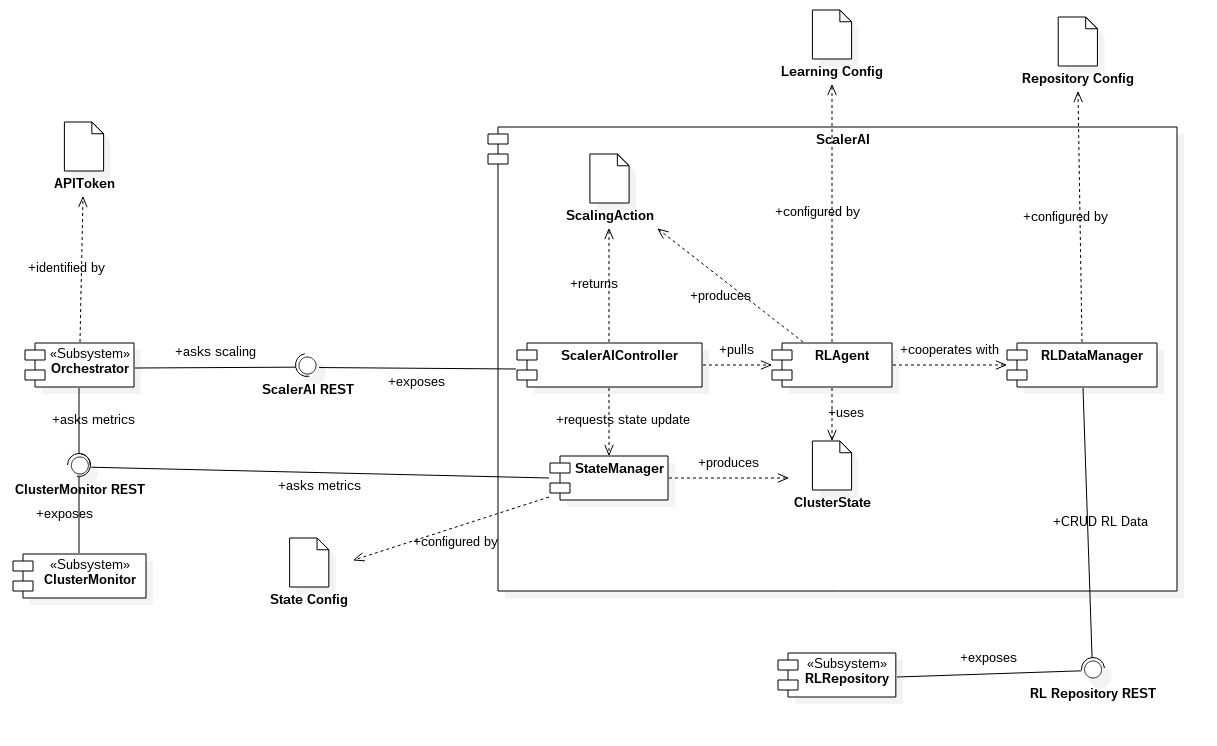
\includegraphics[width=.85\columnwidth]{smart-elasticity-architecture}
	\caption{The architecture.}
\end{figure}
%\vfill
\clearpage
\vfill
\begin{landscape}
	\begin{figure}	
		\label{fig:smart-elasticity-sequence-diagram}
		\centering
		\includegraphics[height=.6\columnwidth, width=.95\columnwidth]{smart-elasticity-sequence-diagram}
		\caption{The auto-scaling activity.}
	\end{figure}
\end{landscape}
\vfill
\clearpage


% %
% REST INTERFACES
% %
\subsection{REST Interfaces}
\label{sec:smart-elasticity-implementation-rest-interfaces}

In this section we detail the REST API exposed by the \texttt{ScalerAI} to manage learning contexts and provide the \texttt{Orchestrator} with the \texttt{ScalingAction}. 
%
Furthermore we detail the REST calls executed by ScalerAI on ClusterMonitor to gather the performance metrics.

\begin{table}
	\label{tbl:smart-elasticity-rest-scalerai}
	\centering
	\begin{tabular}{| m{1.5cm} | m{3cm} | m{3cm} | m{6cm} | }\hline
		
		\textbf{Method} & \textbf{Resource} & \textbf{Params} & \textbf{Description} \\\hline

		\texttt{GET}	& scaling-action    & api-token & Retrieves a new scaling action. \\\hline

		\texttt{GET}    & context           & api-token & Retrieves the learning context. \\\hline
		
		\texttt{PATCH}  & context           & api-token, learningParameters & Modifies the learning context. \\\hline
		
	\end{tabular}
	\caption{The REST interface exposed by \texttt{ScalerAI}.}
\end{table}

\begin{table}
	\label{tbl:smart-elasticity-rest-cluster-monitor}
	\centering
	\begin{tabular}{| m{1.5cm} | m{3cm} | m{3cm} | m{6cm} | }\hline
		
		\textbf{Method} & \textbf{Resource} & \textbf{Params} & \textbf{Description} \\\hline
		
		\texttt{???}	& ???               & ???             & ??? \\\hline
		
		\texttt{???}	& ???               & ???             & ??? \\\hline
				
		\texttt{???}	& ???               & ???             & ??? \\\hline
		
	\end{tabular}
	\caption{The REST interface of interest exposed by Heaster.}
\end{table}